\PassOptionsToPackage{unicode=true}{hyperref} % options for packages loaded elsewhere
\PassOptionsToPackage{hyphens}{url}
%
\documentclass[ignorenonframetext,]{beamer}
\usepackage{pgfpages}
\setbeamertemplate{caption}[numbered]
\setbeamertemplate{caption label separator}{: }
\setbeamercolor{caption name}{fg=normal text.fg}
\beamertemplatenavigationsymbolsempty
% Prevent slide breaks in the middle of a paragraph:
\widowpenalties 1 10000
\raggedbottom
\setbeamertemplate{part page}{
\centering
\begin{beamercolorbox}[sep=16pt,center]{part title}
  \usebeamerfont{part title}\insertpart\par
\end{beamercolorbox}
}
\setbeamertemplate{section page}{
\centering
\begin{beamercolorbox}[sep=12pt,center]{part title}
  \usebeamerfont{section title}\insertsection\par
\end{beamercolorbox}
}
\setbeamertemplate{subsection page}{
\centering
\begin{beamercolorbox}[sep=8pt,center]{part title}
  \usebeamerfont{subsection title}\insertsubsection\par
\end{beamercolorbox}
}
\AtBeginPart{
  \frame{\partpage}
}
\AtBeginSection{
  \ifbibliography
  \else
    \frame{\sectionpage}
  \fi
}
\AtBeginSubsection{
  \frame{\subsectionpage}
}
\usepackage{lmodern}
\usepackage{amssymb,amsmath}
\usepackage{ifxetex,ifluatex}
\usepackage{fixltx2e} % provides \textsubscript
\ifnum 0\ifxetex 1\fi\ifluatex 1\fi=0 % if pdftex
  \usepackage[T1]{fontenc}
  \usepackage[utf8]{inputenc}
  \usepackage{textcomp} % provides euro and other symbols
\else % if luatex or xelatex
  \usepackage{unicode-math}
  \defaultfontfeatures{Ligatures=TeX,Scale=MatchLowercase}
\fi
% use upquote if available, for straight quotes in verbatim environments
\IfFileExists{upquote.sty}{\usepackage{upquote}}{}
% use microtype if available
\IfFileExists{microtype.sty}{%
\usepackage[]{microtype}
\UseMicrotypeSet[protrusion]{basicmath} % disable protrusion for tt fonts
}{}
\IfFileExists{parskip.sty}{%
\usepackage{parskip}
}{% else
\setlength{\parindent}{0pt}
\setlength{\parskip}{6pt plus 2pt minus 1pt}
}
\usepackage{hyperref}
\hypersetup{
            pdftitle={Regression with many features},
            pdfborder={0 0 0},
            breaklinks=true}
\urlstyle{same}  % don't use monospace font for urls
\newif\ifbibliography
\setlength{\emergencystretch}{3em}  % prevent overfull lines
\providecommand{\tightlist}{%
  \setlength{\itemsep}{0pt}\setlength{\parskip}{0pt}}
\setcounter{secnumdepth}{0}

% set default figure placement to htbp
\makeatletter
\def\fps@figure{htbp}
\makeatother


\title{Regression with many features}
\author{}
\date{\vspace{-2.5em}}

\begin{document}
\frame{\titlepage}

\begin{frame}{An example of a strong linear association between a
continuous phenotype (age) on the x-axis and a feature of interest (gene
expression for a given gene) on the y-axis. A strong linear relationship
with a positive slope exists between the two.}
\protect\hypertarget{an-example-of-a-strong-linear-association-between-a-continuous-phenotype-age-on-the-x-axis-and-a-feature-of-interest-gene-expression-for-a-given-gene-on-the-y-axis.-a-strong-linear-relationship-with-a-positive-slope-exists-between-the-two.}{}

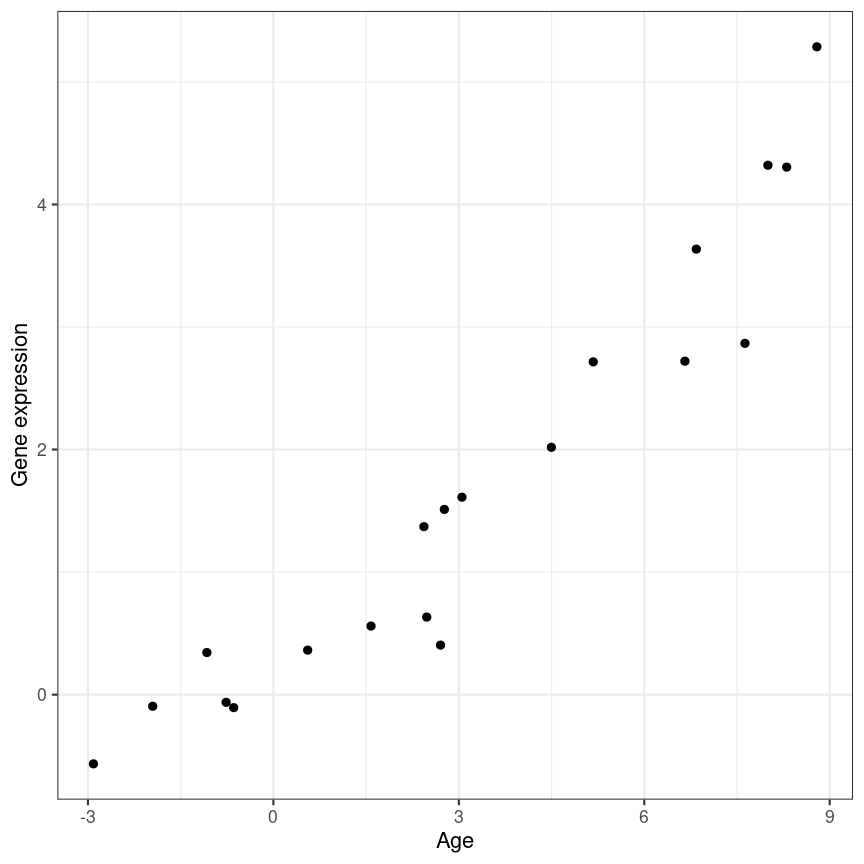
\includegraphics[width=0.5\textwidth]{/home/runner/work/high-dimensional-stats-r/high-dimensional-stats-r/fig/rmd-02-unnamed-chunk-2-1}



\end{frame}

\begin{frame}{An example of a strong linear association between a
discrete phenotype (group) on the x-axis and a feature of interest (gene
expression for a given gene) on the y-axis. The two groups clearly
differ with respect to gene expression.}
\protect\hypertarget{an-example-of-a-strong-linear-association-between-a-discrete-phenotype-group-on-the-x-axis-and-a-feature-of-interest-gene-expression-for-a-given-gene-on-the-y-axis.-the-two-groups-clearly-differ-with-respect-to-gene-expression.}{}

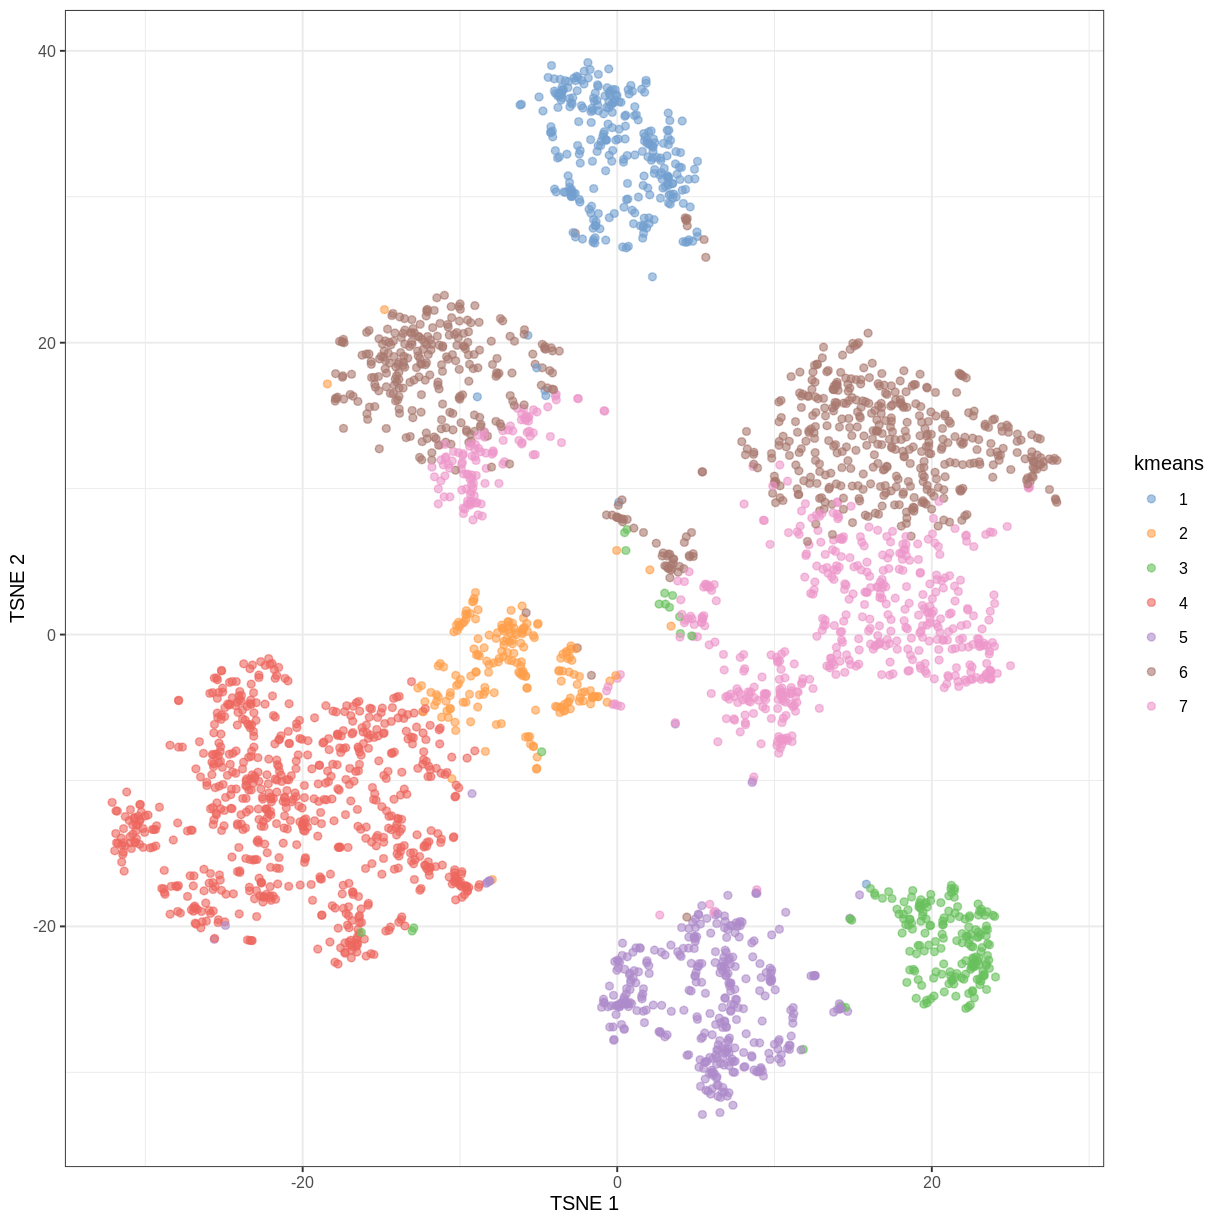
\includegraphics[width=0.5\textwidth]{/home/runner/work/high-dimensional-stats-r/high-dimensional-stats-r/fig/rmd-02-unnamed-chunk-3-1}



\end{frame}

\begin{frame}{An example of a strong linear association between a
discrete phenotype (group) on the x-axis and a feature of interest (gene
expression for a given gene) on the y-axis. The two groups seem to
differ with respect to gene expression, but the relationship is weak.}
\protect\hypertarget{an-example-of-a-strong-linear-association-between-a-discrete-phenotype-group-on-the-x-axis-and-a-feature-of-interest-gene-expression-for-a-given-gene-on-the-y-axis.-the-two-groups-seem-to-differ-with-respect-to-gene-expression-but-the-relationship-is-weak.}{}

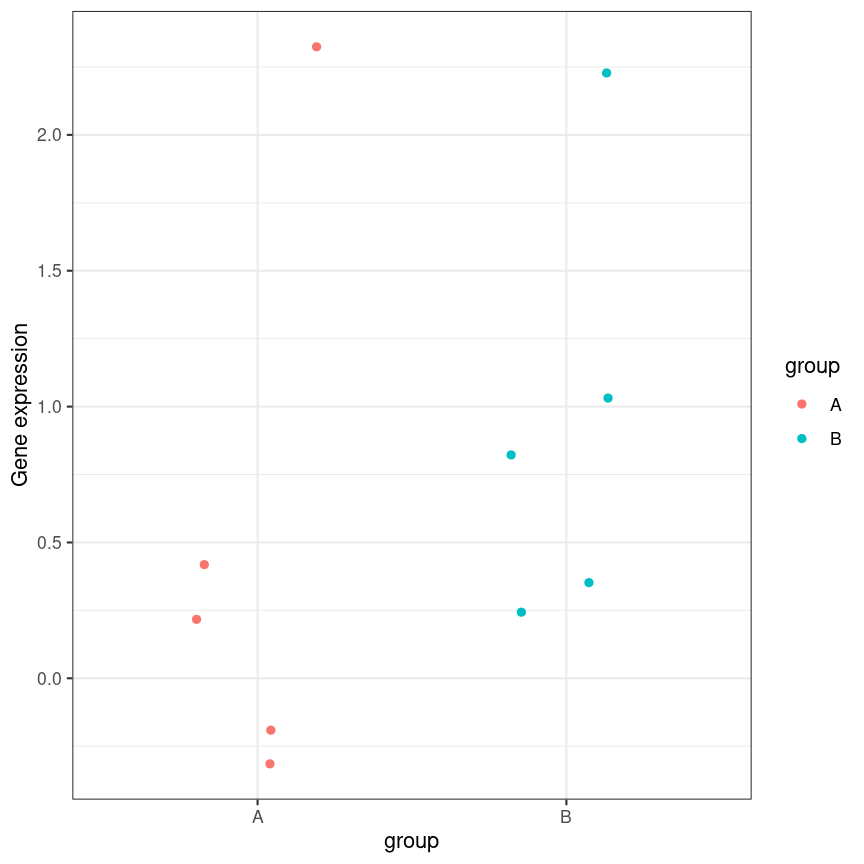
\includegraphics[width=0.5\textwidth]{/home/runner/work/high-dimensional-stats-r/high-dimensional-stats-r/fig/rmd-02-unnamed-chunk-4-1}



\end{frame}

\begin{frame}{The generative model of a simple linear regression with a
fixed slope and intercept. Lightly shaded regions represent regions
where observations are probable, and darker regions represent lower
probability.}
\protect\hypertarget{the-generative-model-of-a-simple-linear-regression-with-a-fixed-slope-and-intercept.-lightly-shaded-regions-represent-regions-where-observations-are-probable-and-darker-regions-represent-lower-probability.}{}

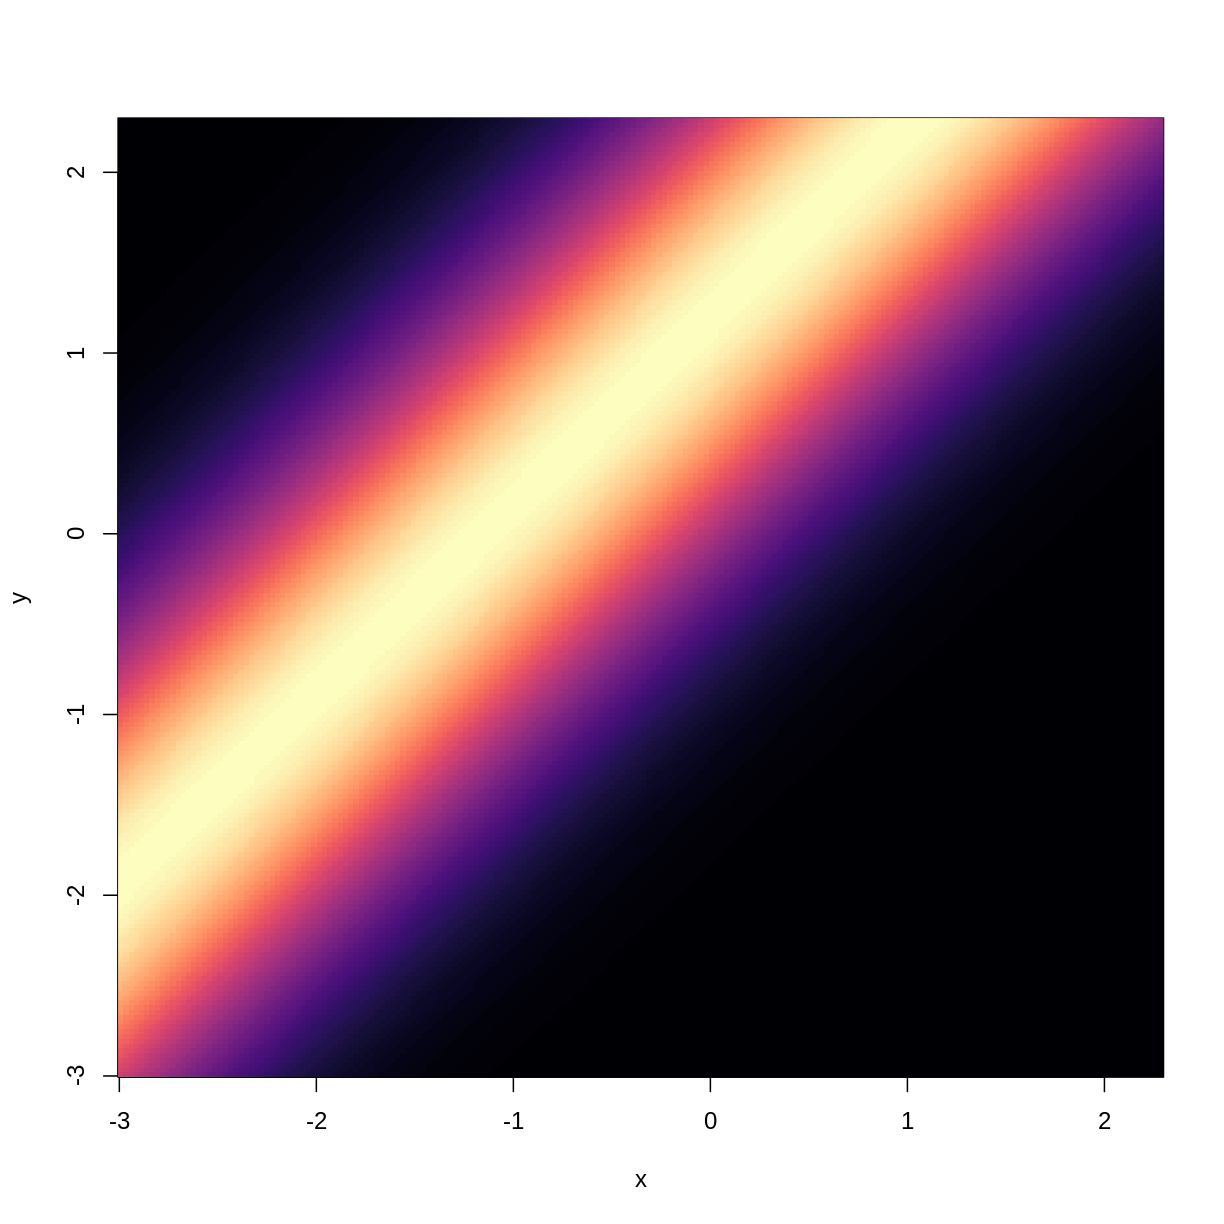
\includegraphics[width=0.5\textwidth]{/home/runner/work/high-dimensional-stats-r/high-dimensional-stats-r/fig/rmd-02-unnamed-chunk-5-1}



\end{frame}

\begin{frame}{Density plot of a t-distribution showing the observed test
statistics (here, t-statistics). The p-values, visualised here with
shaded regions, represent the portion of the null distribution that is
as extreme or more extreme as the observed test statistics, which are
shown as dashed lines.}
\protect\hypertarget{density-plot-of-a-t-distribution-showing-the-observed-test-statistics-here-t-statistics.-the-p-values-visualised-here-with-shaded-regions-represent-the-portion-of-the-null-distribution-that-is-as-extreme-or-more-extreme-as-the-observed-test-statistics-which-are-shown-as-dashed-lines.}{}

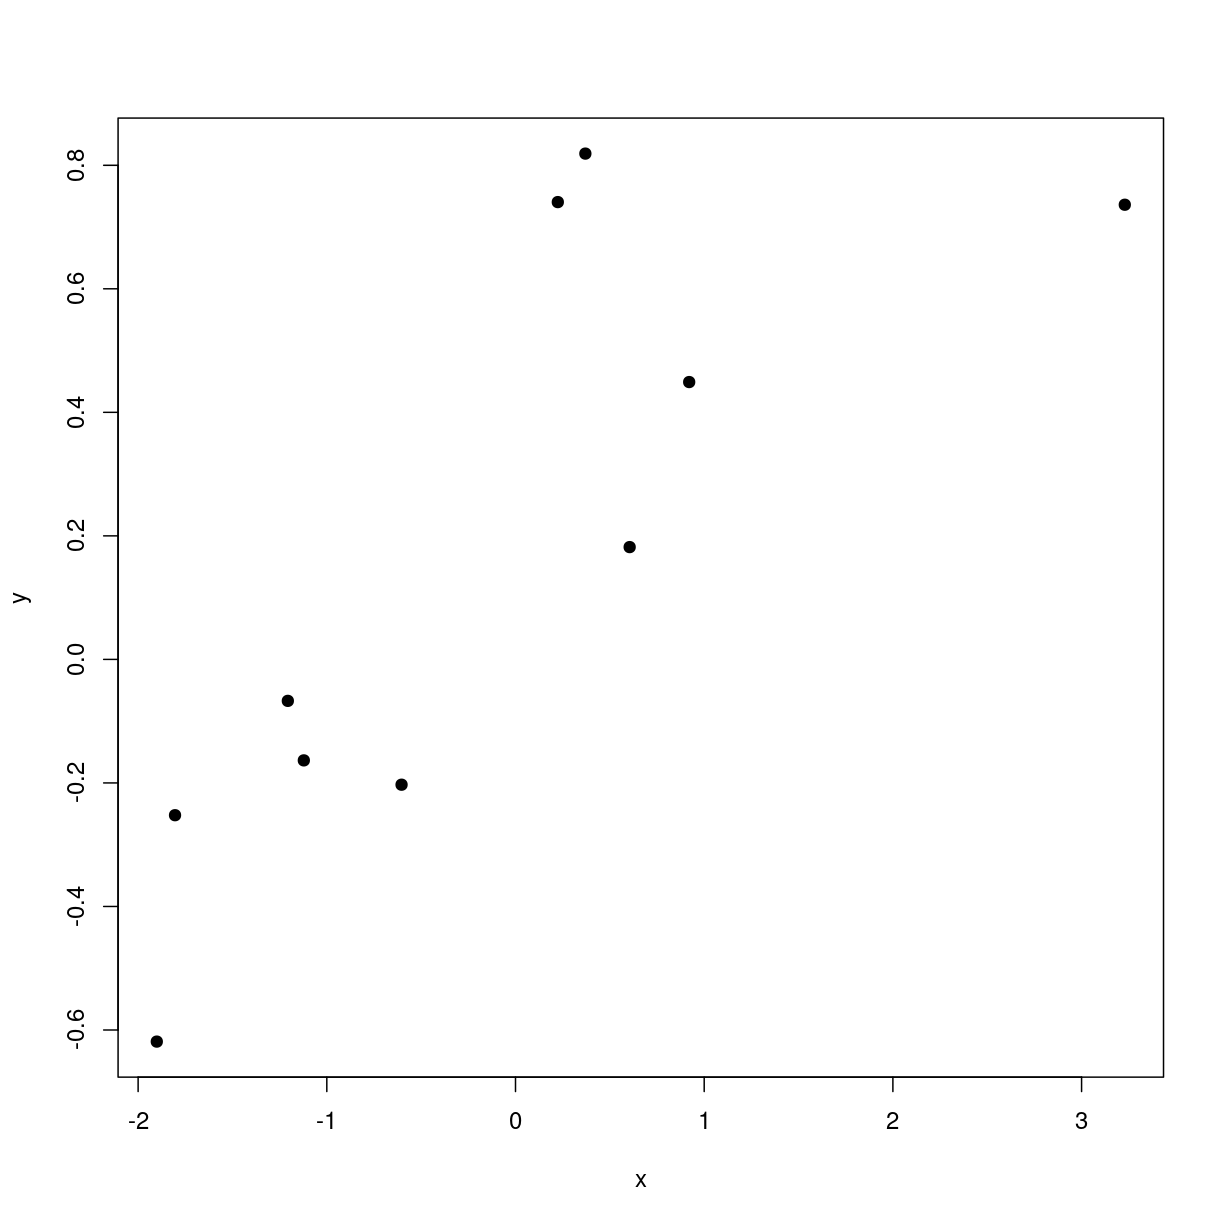
\includegraphics[width=0.5\textwidth]{/home/runner/work/high-dimensional-stats-r/high-dimensional-stats-r/fig/rmd-02-unnamed-chunk-9-1}



\end{frame}

\begin{frame}{An example of a linear relationship for 100 points with a
small amount of noise and small effect sizes that is statistically
significant.}
\protect\hypertarget{an-example-of-a-linear-relationship-for-100-points-with-a-small-amount-of-noise-and-small-effect-sizes-that-is-statistically-significant.}{}

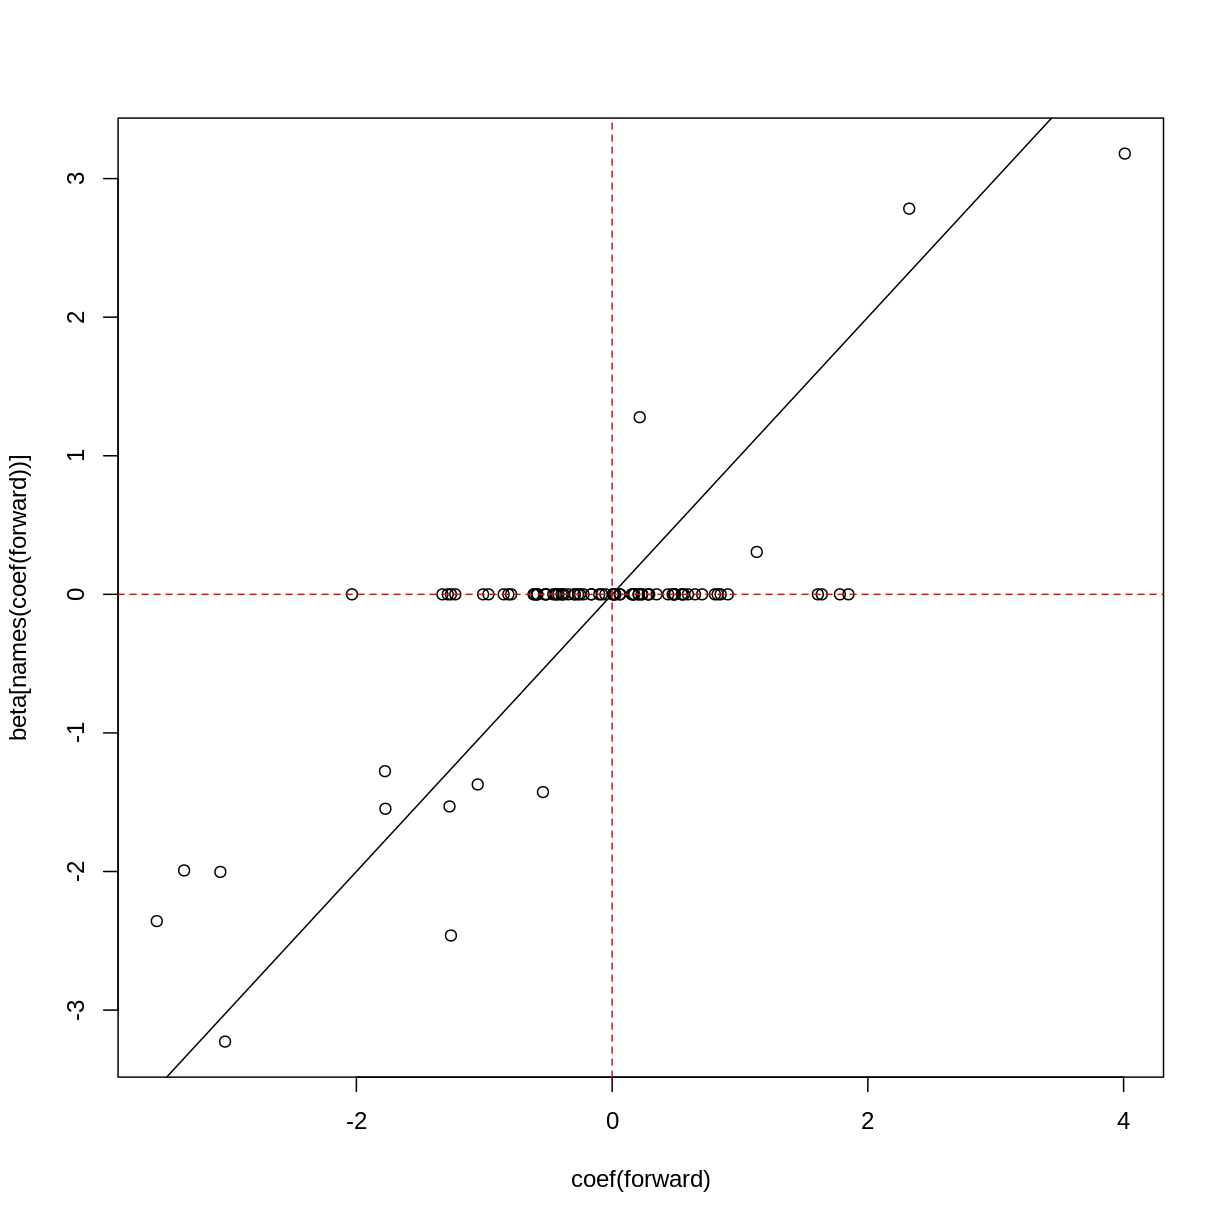
\includegraphics[width=0.5\textwidth]{/home/runner/work/high-dimensional-stats-r/high-dimensional-stats-r/fig/rmd-02-unnamed-chunk-10-1}



\end{frame}

\begin{frame}{An example of a linear relationship for 100 points with a
large amount of noise and large effect sizes that is not statistically
significant.}
\protect\hypertarget{an-example-of-a-linear-relationship-for-100-points-with-a-large-amount-of-noise-and-large-effect-sizes-that-is-not-statistically-significant.}{}

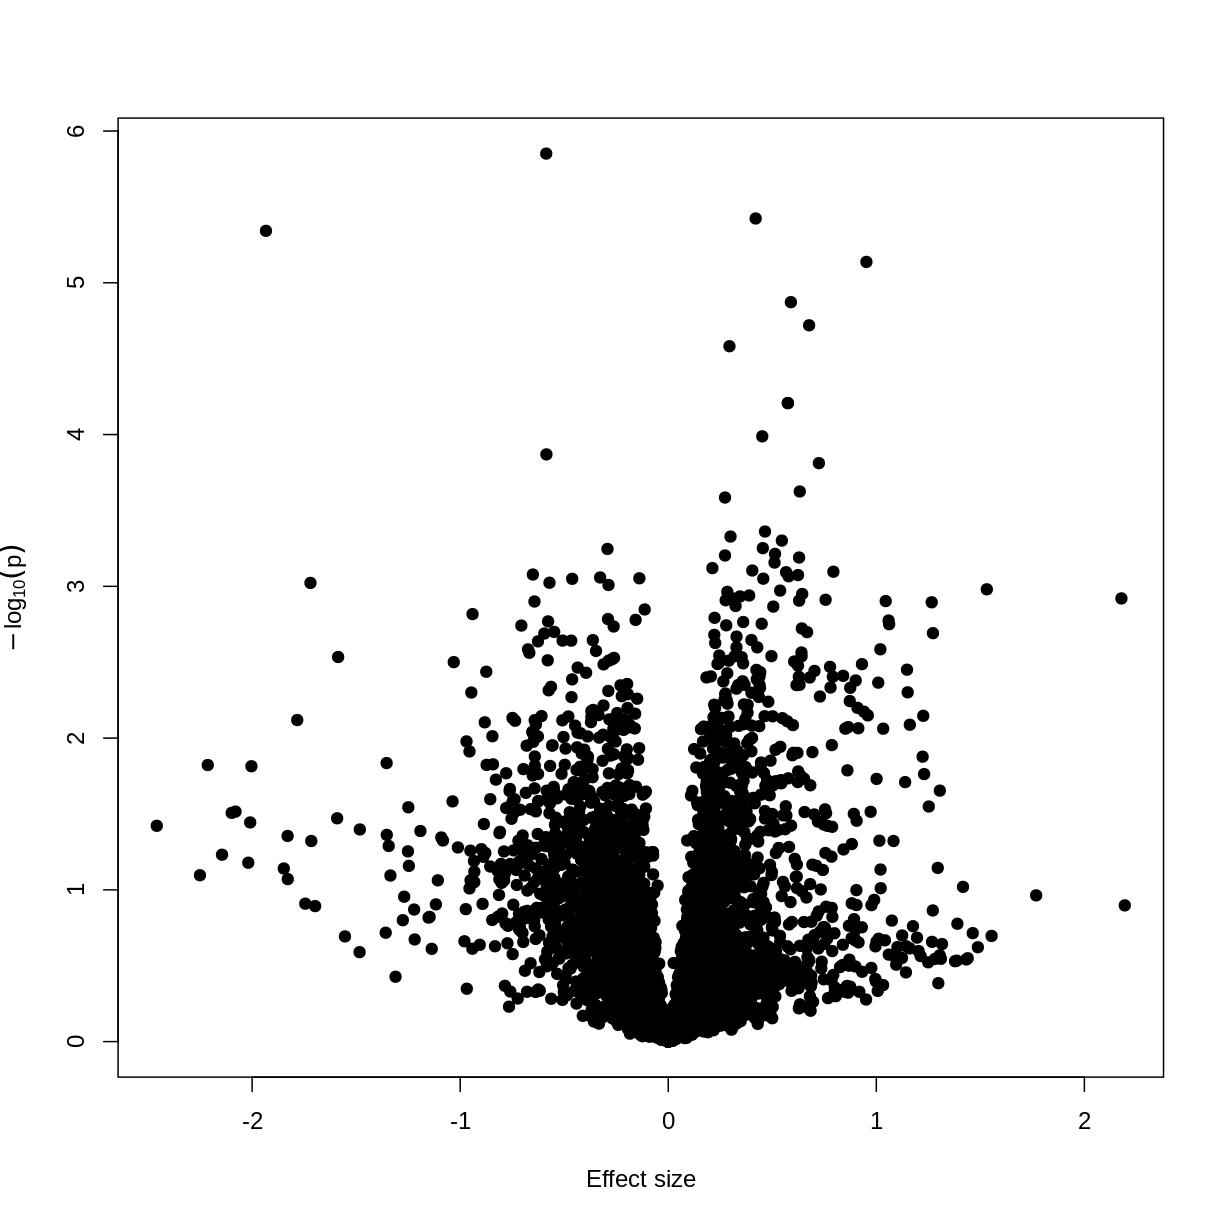
\includegraphics[width=0.5\textwidth]{/home/runner/work/high-dimensional-stats-r/high-dimensional-stats-r/fig/rmd-02-unnamed-chunk-11-1}



\end{frame}

\begin{frame}{An example of a linear relationship for 10 points with a
large amount of noise and large effect sizes that is not statistically
significant.}
\protect\hypertarget{an-example-of-a-linear-relationship-for-10-points-with-a-large-amount-of-noise-and-large-effect-sizes-that-is-not-statistically-significant.}{}

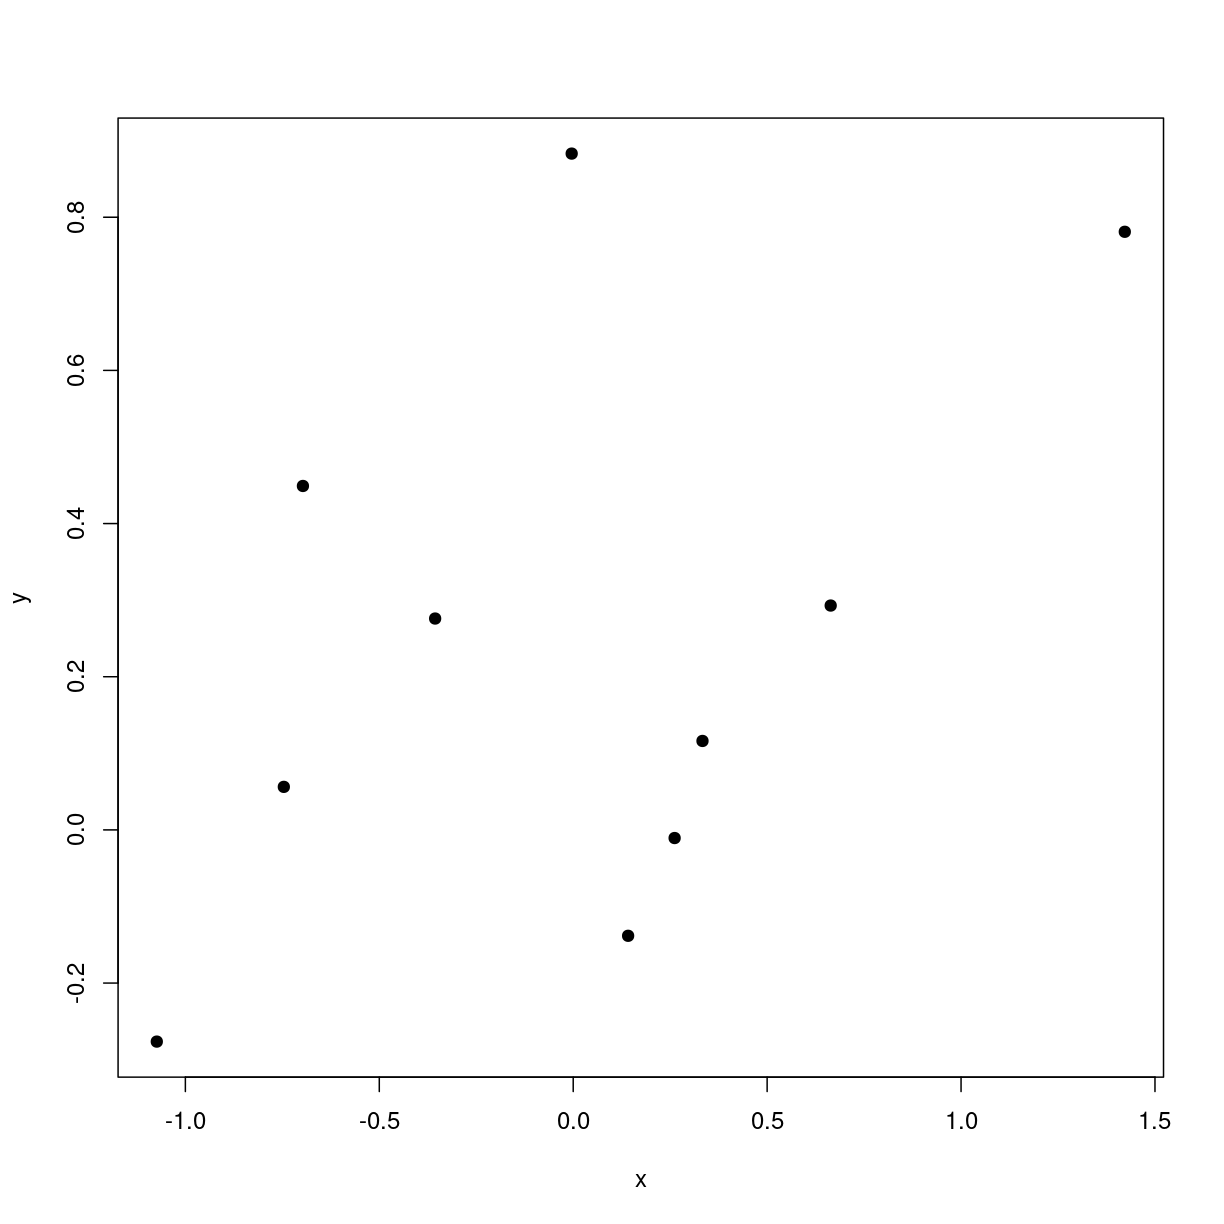
\includegraphics[width=0.5\textwidth]{/home/runner/work/high-dimensional-stats-r/high-dimensional-stats-r/fig/rmd-02-unnamed-chunk-12-1}



\end{frame}

\begin{frame}{An example of a linear relationship for 10 points with a
small amount of noise and small effect sizes that is statistically
significant.}
\protect\hypertarget{an-example-of-a-linear-relationship-for-10-points-with-a-small-amount-of-noise-and-small-effect-sizes-that-is-statistically-significant.}{}

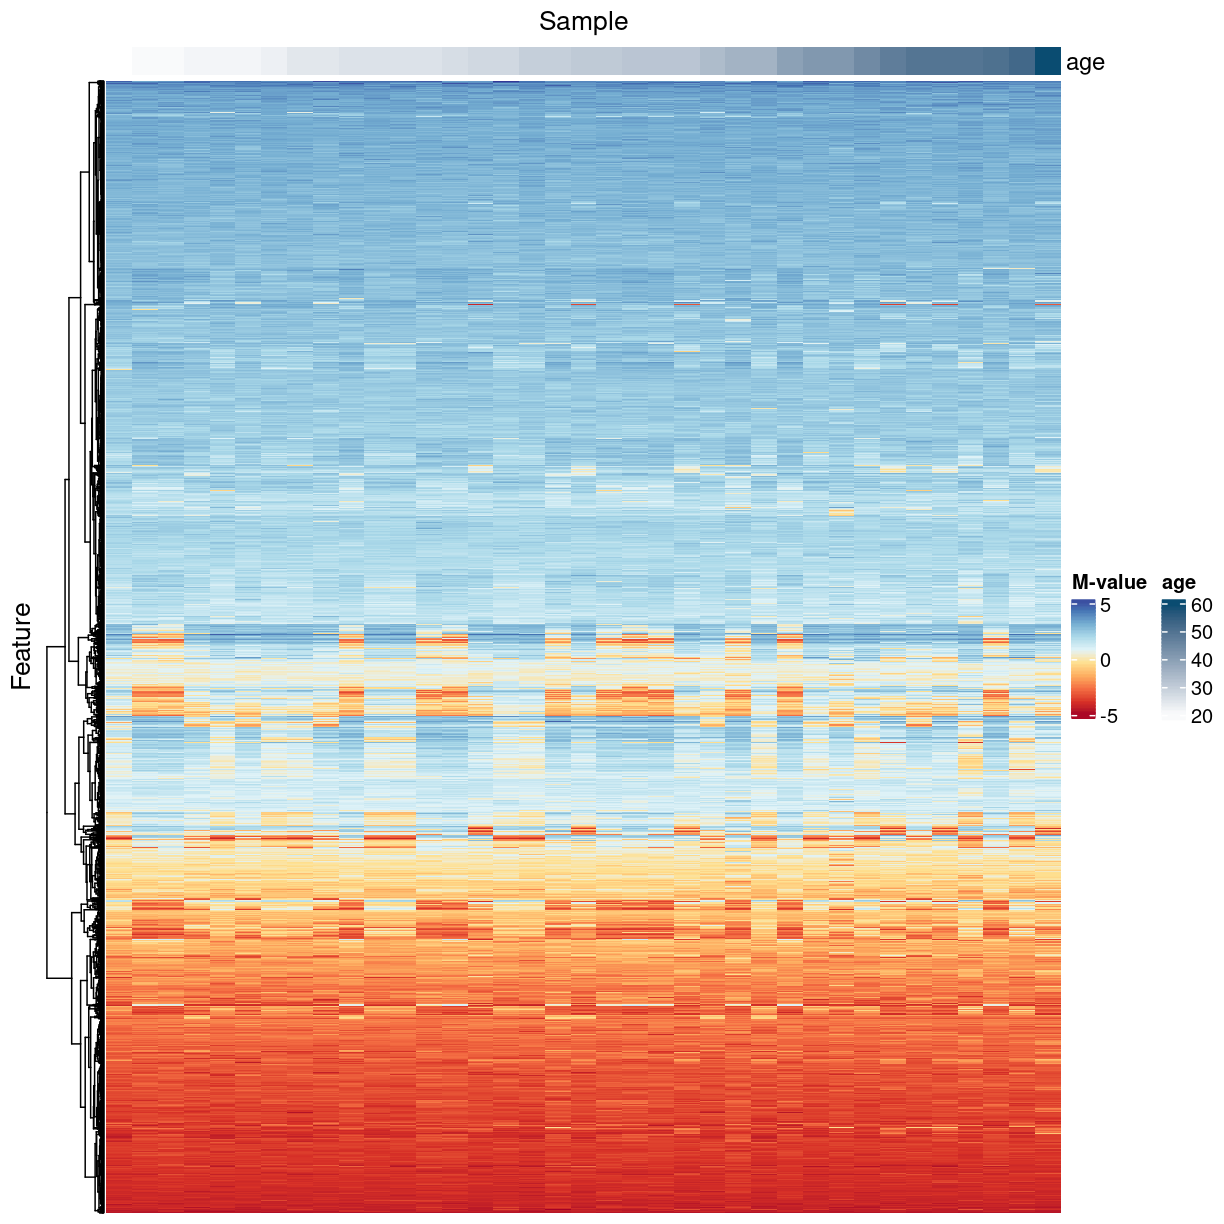
\includegraphics[width=0.5\textwidth]{/home/runner/work/high-dimensional-stats-r/high-dimensional-stats-r/fig/rmd-02-unnamed-chunk-13-1}



\end{frame}

\begin{frame}{An example of a linear relationship for 1,000 points with
a large amount of noise and small effect sizes that is statistically
significant.}
\protect\hypertarget{an-example-of-a-linear-relationship-for-1000-points-with-a-large-amount-of-noise-and-small-effect-sizes-that-is-statistically-significant.}{}

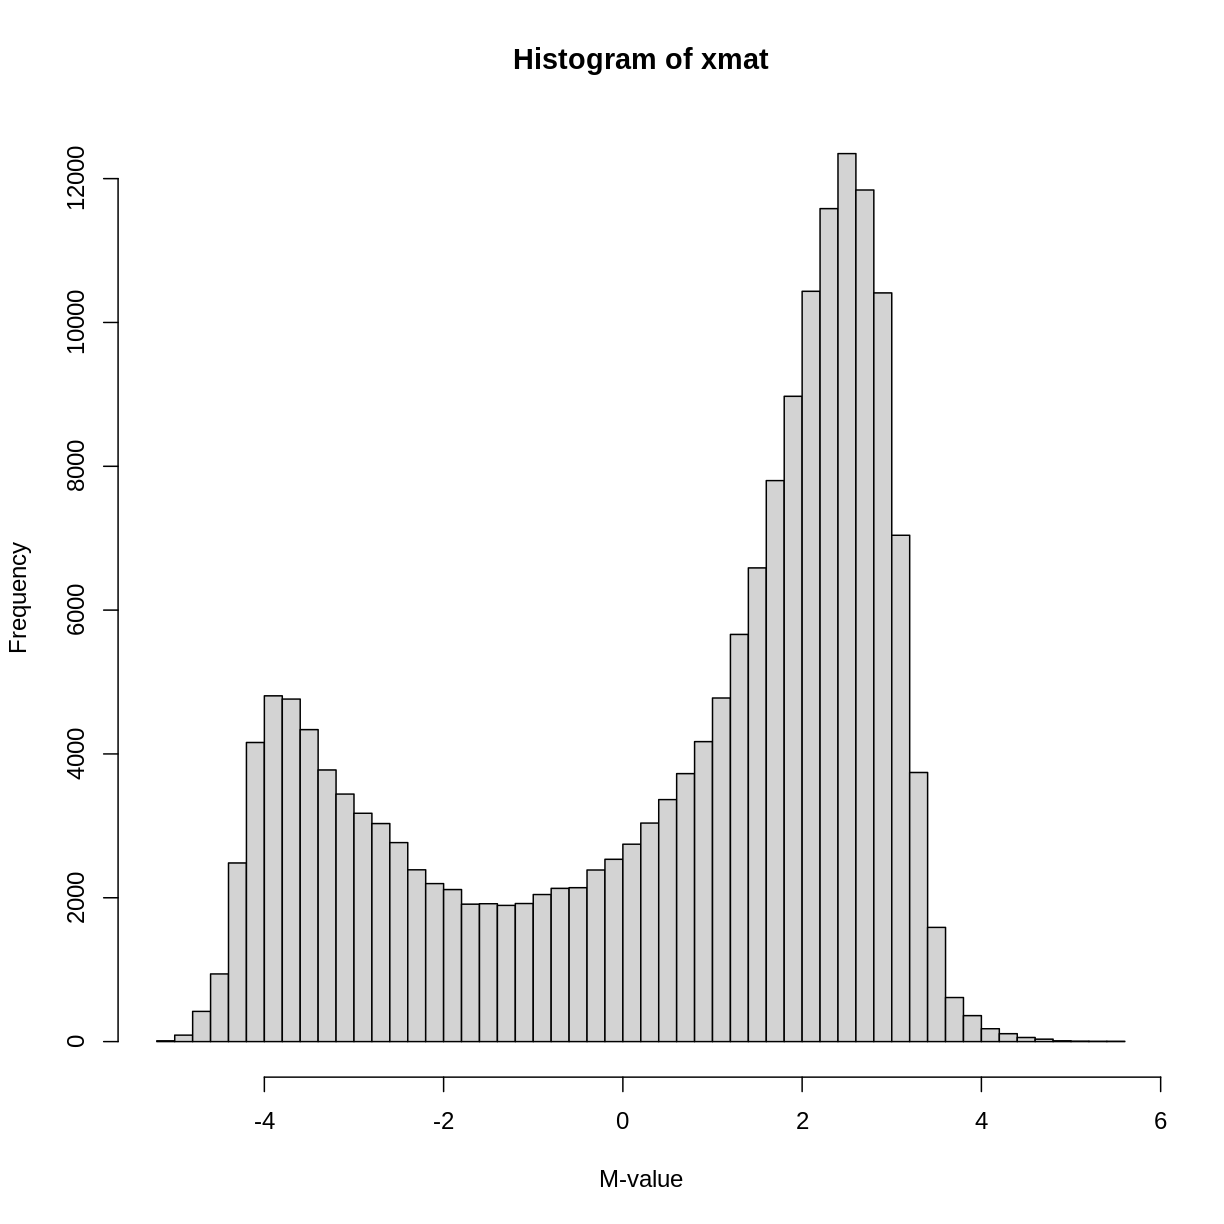
\includegraphics[width=0.5\textwidth]{/home/runner/work/high-dimensional-stats-r/high-dimensional-stats-r/fig/rmd-02-unnamed-chunk-14-1}



\end{frame}

\begin{frame}{An example of a linear relationship for 1,000 points with
a small amount of noise and small effect sizes that is statistically
significant.}
\protect\hypertarget{an-example-of-a-linear-relationship-for-1000-points-with-a-small-amount-of-noise-and-small-effect-sizes-that-is-statistically-significant.}{}

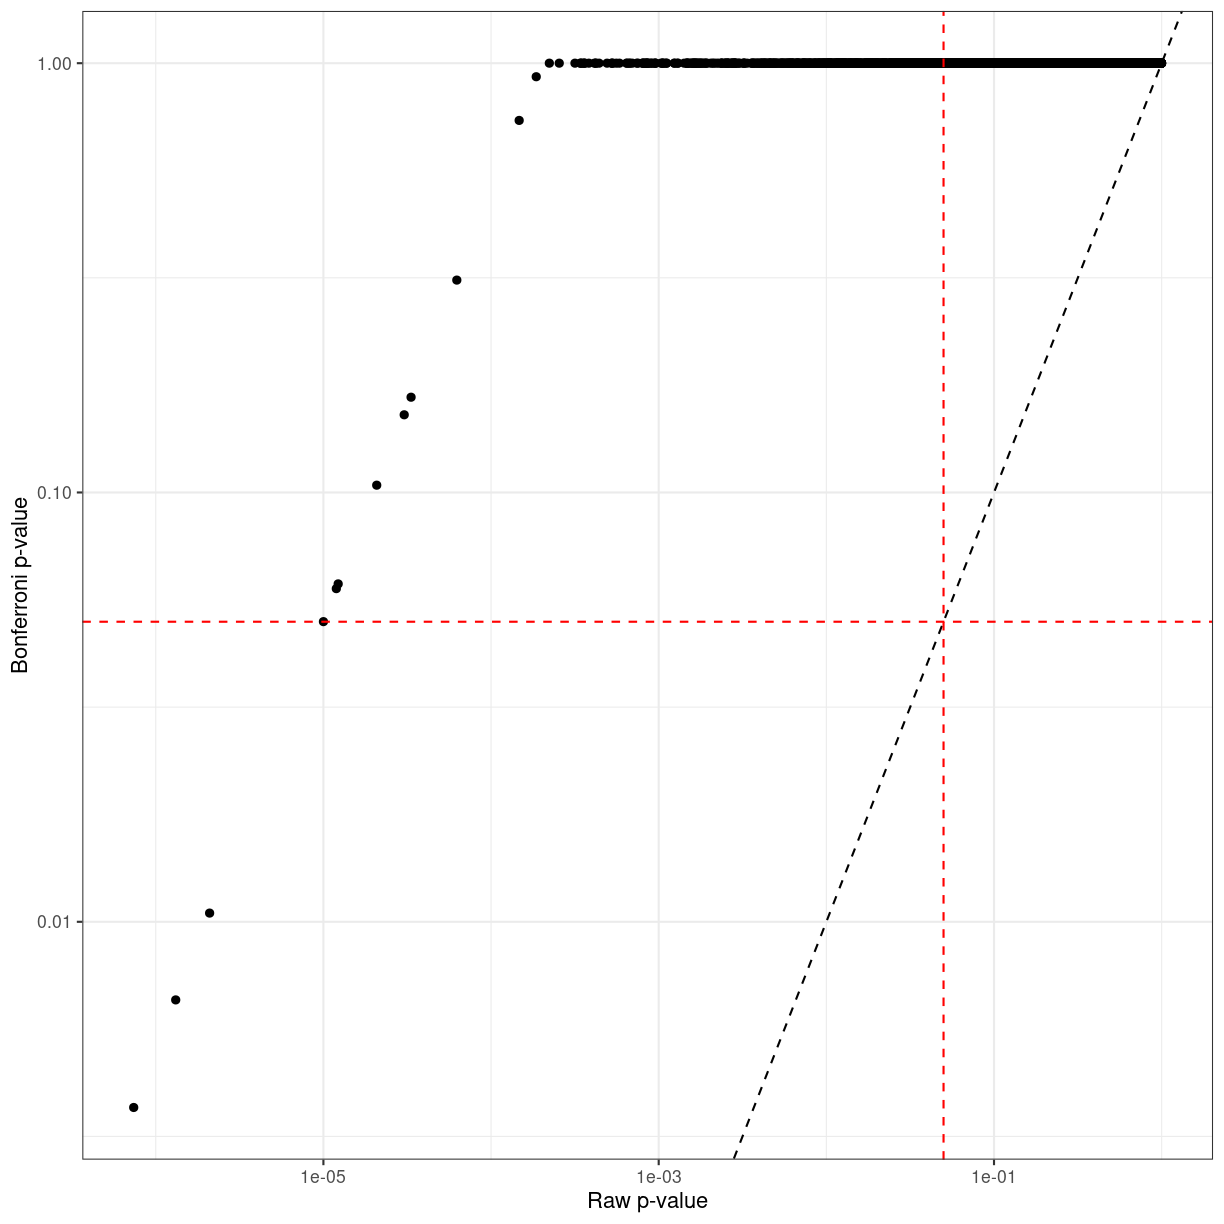
\includegraphics[width=0.5\textwidth]{/home/runner/work/high-dimensional-stats-r/high-dimensional-stats-r/fig/rmd-02-unnamed-chunk-15-1}



\end{frame}

\begin{frame}{Histogram of M-values for all features. The distribution
appears to be bimodal, with a large number of unmethylated features as
well as many methylated features, and many intermediate features.}
\protect\hypertarget{histogram-of-m-values-for-all-features.-the-distribution-appears-to-be-bimodal-with-a-large-number-of-unmethylated-features-as-well-as-many-methylated-features-and-many-intermediate-features.}{}

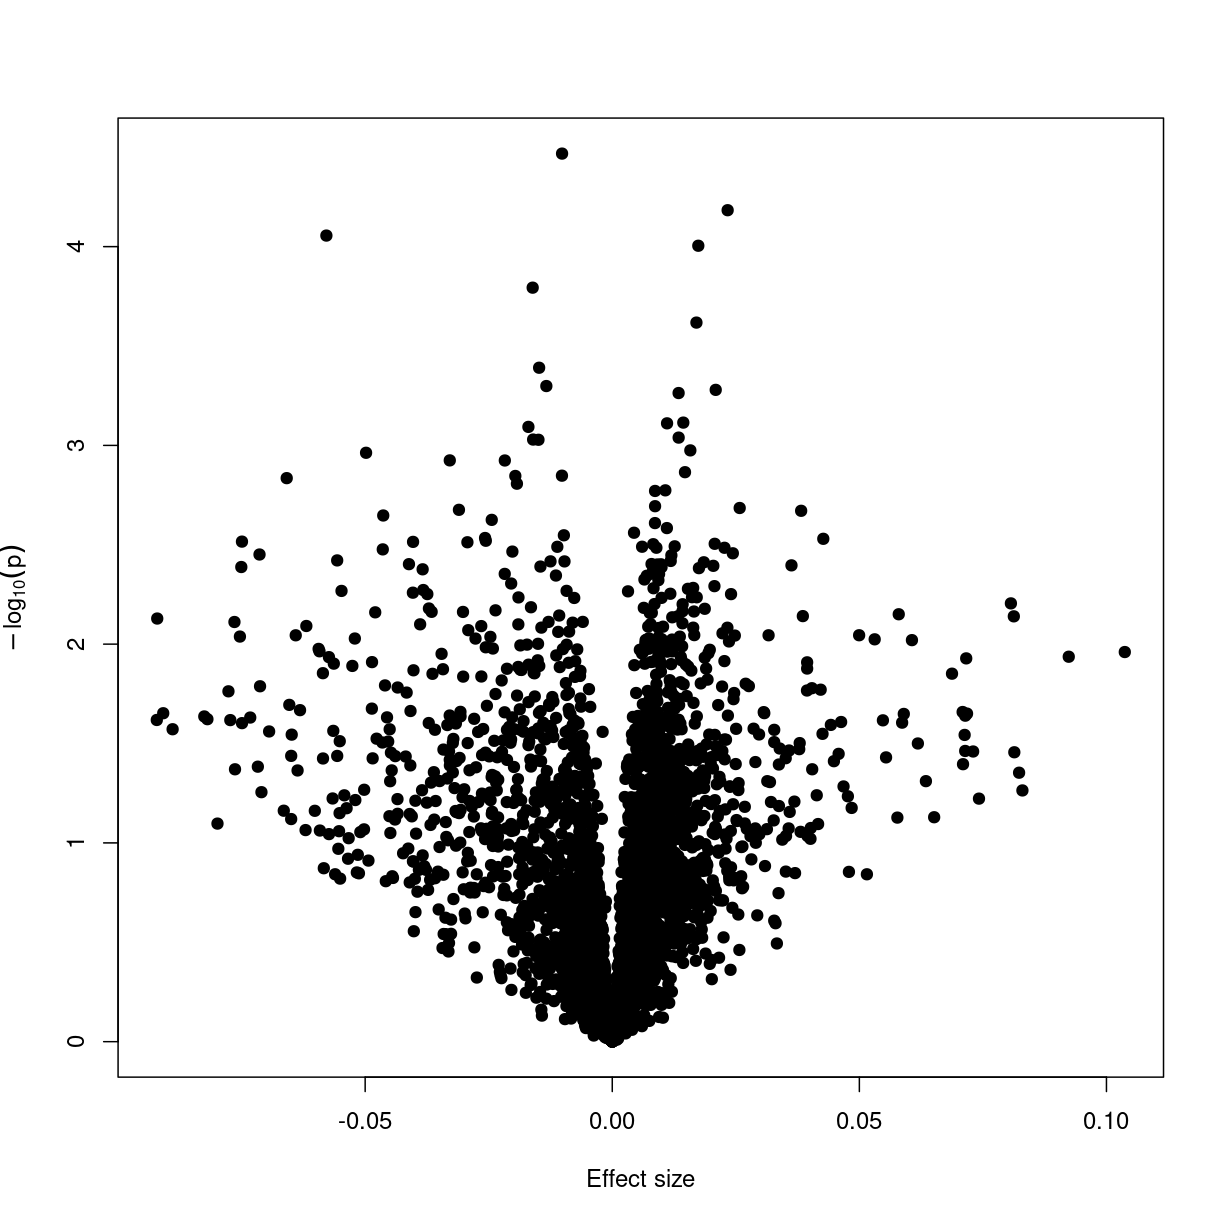
\includegraphics[width=0.5\textwidth]{/home/runner/work/high-dimensional-stats-r/high-dimensional-stats-r/fig/rmd-02-unnamed-chunk-20-1}



\end{frame}

\begin{frame}{Heatmap of methylation values across all features. Samples
are ordered according to age.}
\protect\hypertarget{heatmap-of-methylation-values-across-all-features.-samples-are-ordered-according-to-age.}{}

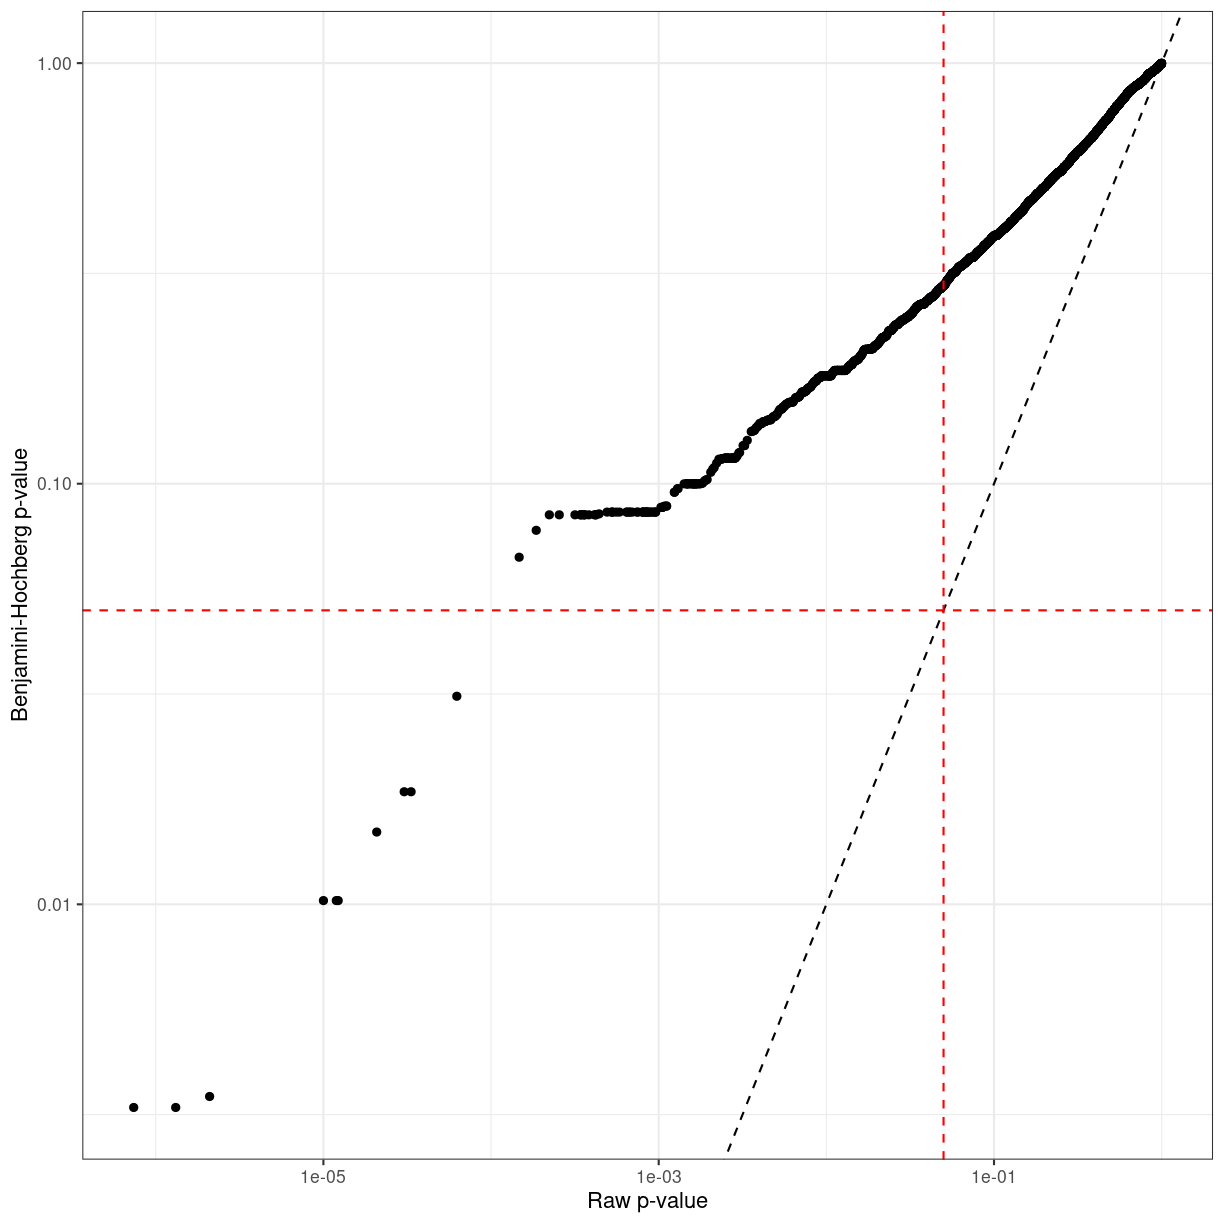
\includegraphics[width=0.5\textwidth]{/home/runner/work/high-dimensional-stats-r/high-dimensional-stats-r/fig/rmd-02-unnamed-chunk-22-1}



\end{frame}

\begin{frame}{Plot of -log10(p) against effect size estimates for a
regression of age against methylation level for each feature in the
data.}
\protect\hypertarget{plot-of--log10p-against-effect-size-estimates-for-a-regression-of-age-against-methylation-level-for-each-feature-in-the-data.}{}

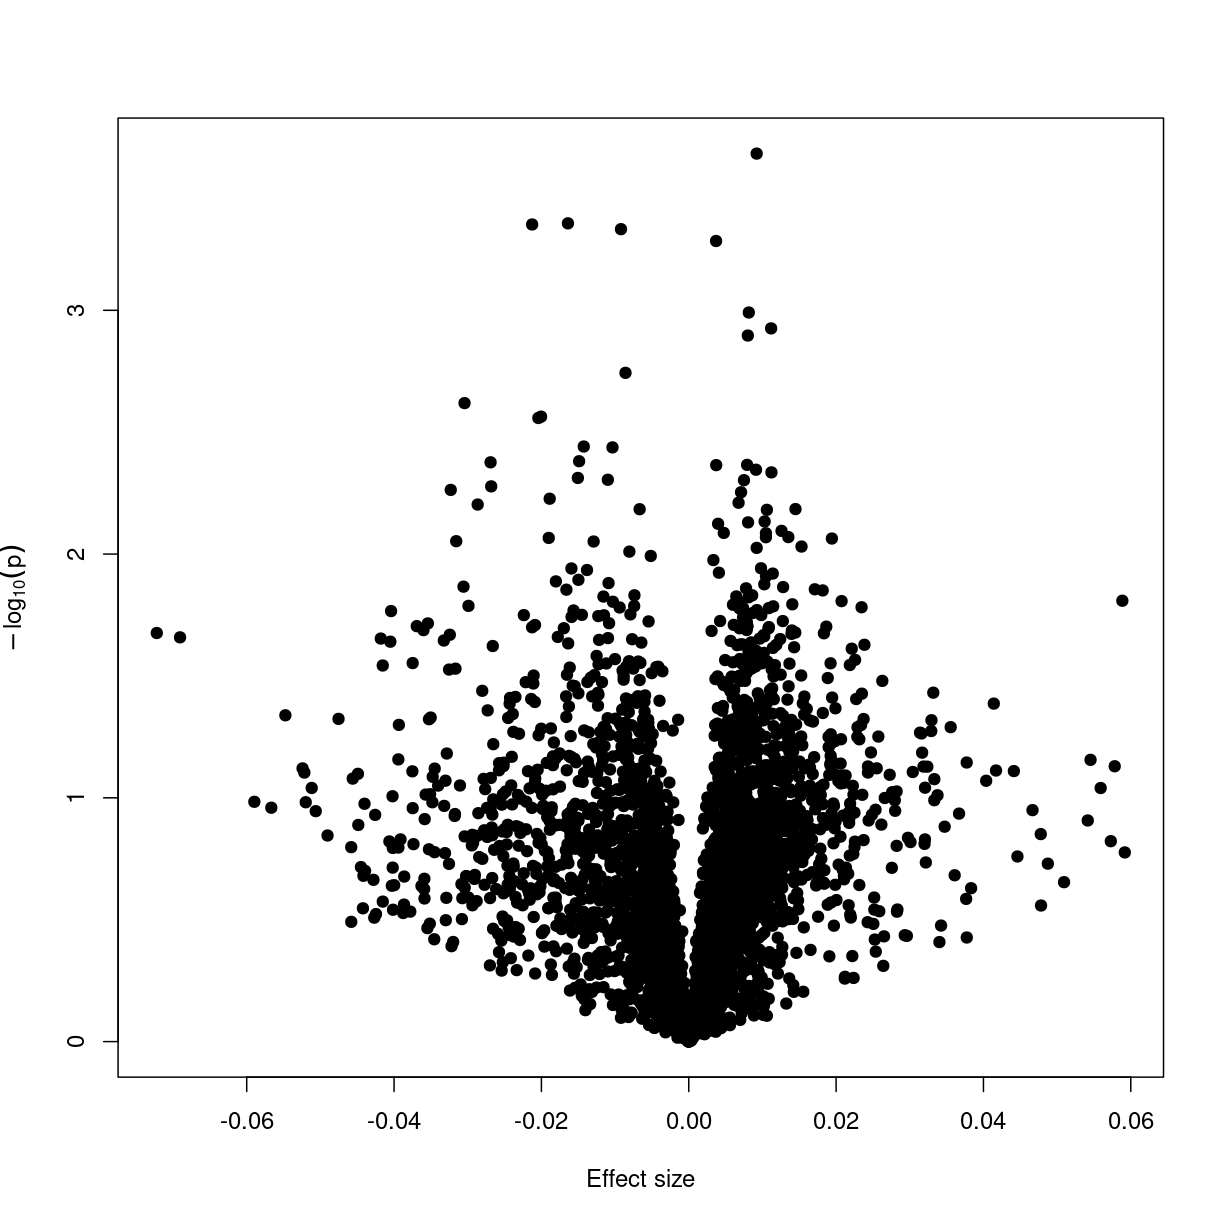
\includegraphics[width=0.5\textwidth]{/home/runner/work/high-dimensional-stats-r/high-dimensional-stats-r/fig/rmd-02-unnamed-chunk-29-1}



\end{frame}

\begin{frame}{Plot of -log10(p) against effect size estimates for a
regression of a made-up feature against methylation level for each
feature in the data. A dashed line represents a 0.05 significance
level.}
\protect\hypertarget{plot-of--log10p-against-effect-size-estimates-for-a-regression-of-a-made-up-feature-against-methylation-level-for-each-feature-in-the-data.-a-dashed-line-represents-a-0.05-significance-level.}{}

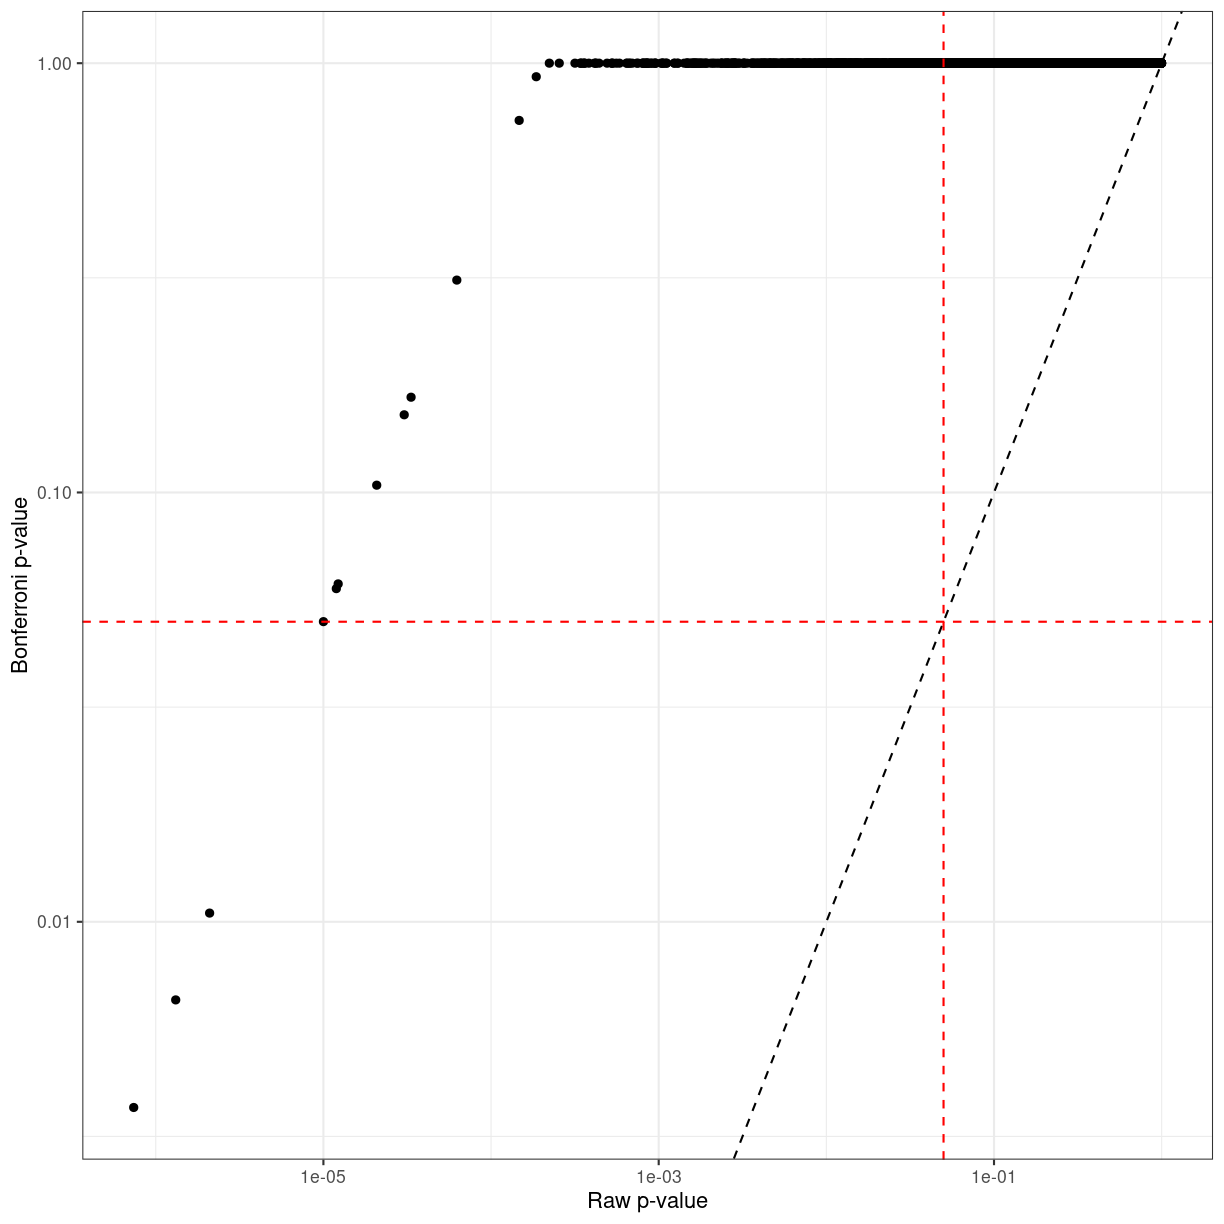
\includegraphics[width=0.5\textwidth]{/home/runner/work/high-dimensional-stats-r/high-dimensional-stats-r/fig/rmd-02-unnamed-chunk-30-1}



\end{frame}

\begin{frame}{Plot of Bonferroni-adjusted p-values (y) against
unadjusted p-values (x). A dashed black line represents the identity
(where x=y), while dashed red lines represent 0.05 significance
thresholds.}
\protect\hypertarget{plot-of-bonferroni-adjusted-p-values-y-against-unadjusted-p-values-x.-a-dashed-black-line-represents-the-identity-where-xy-while-dashed-red-lines-represent-0.05-significance-thresholds.}{}

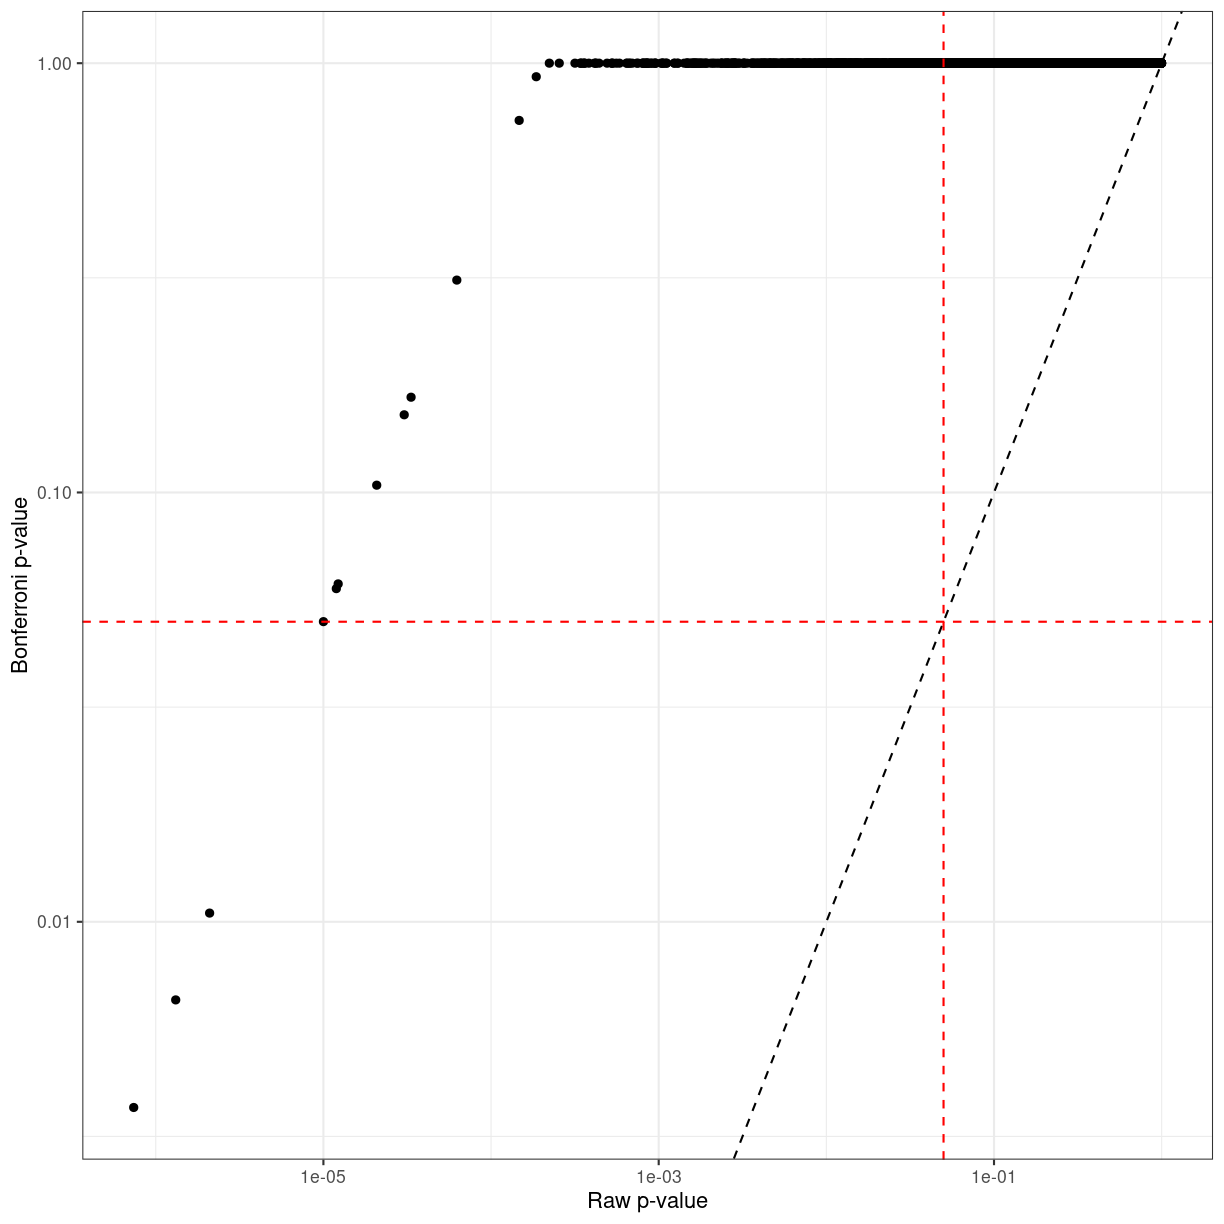
\includegraphics[width=0.5\textwidth]{/home/runner/work/high-dimensional-stats-r/high-dimensional-stats-r/fig/rmd-02-unnamed-chunk-31-1}



\end{frame}

\begin{frame}{Plot of Benjamini-Hochberg-adjusted p-values (y) against
unadjusted p-values (x). A dashed black line represents the identity
(where x=y), while dashed red lines represent 0.05 significance
thresholds.}
\protect\hypertarget{plot-of-benjamini-hochberg-adjusted-p-values-y-against-unadjusted-p-values-x.-a-dashed-black-line-represents-the-identity-where-xy-while-dashed-red-lines-represent-0.05-significance-thresholds.}{}

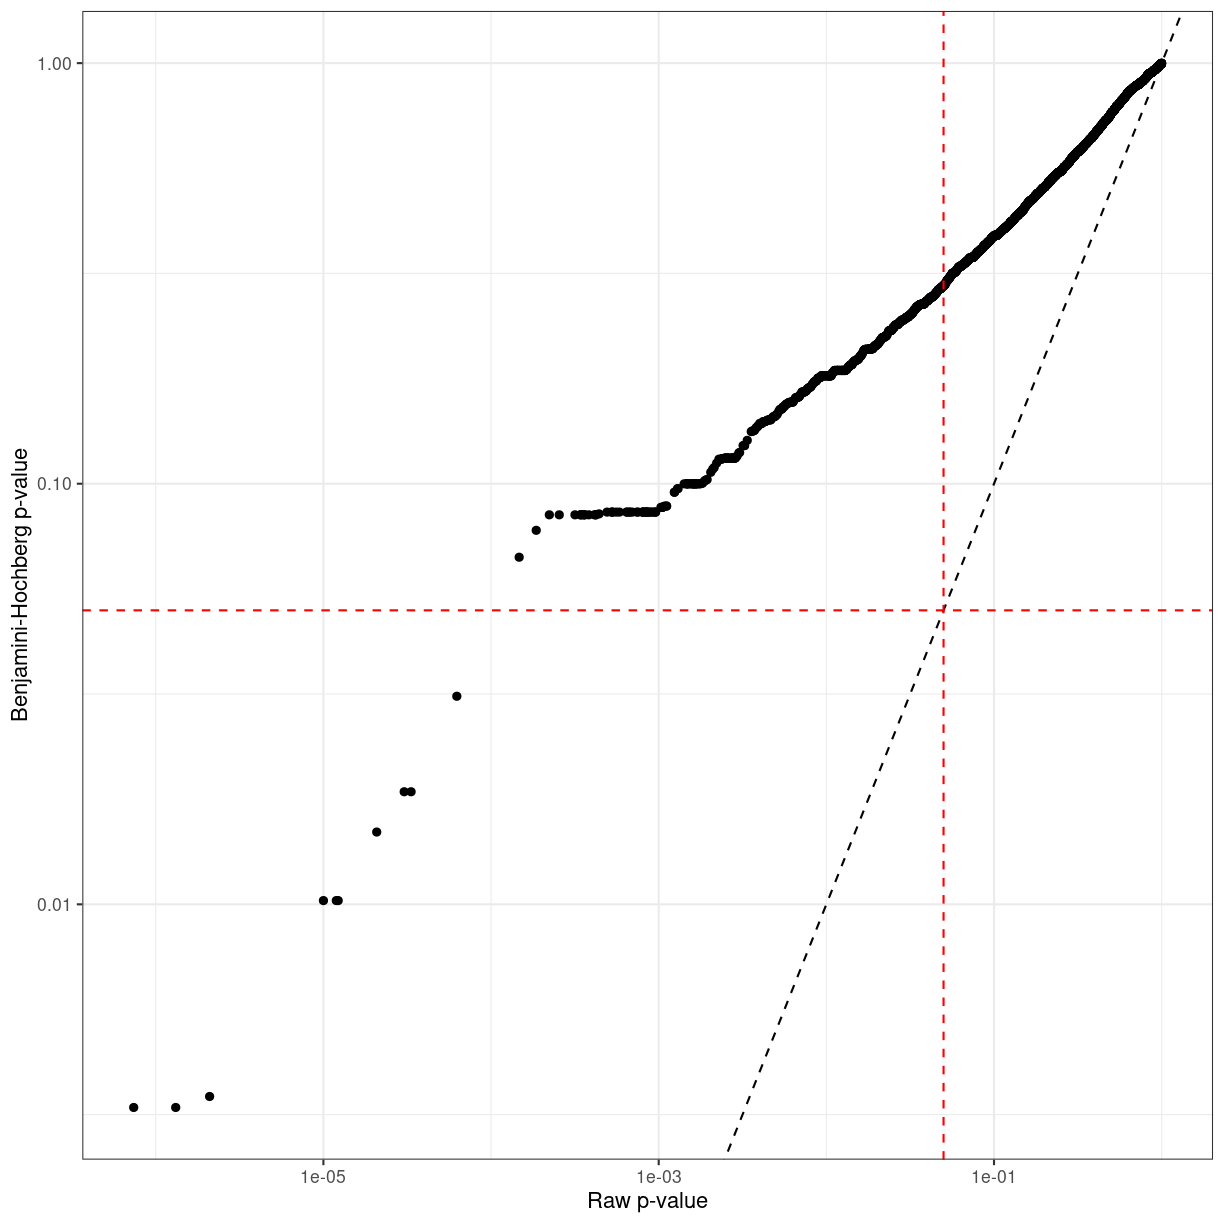
\includegraphics[width=0.5\textwidth]{/home/runner/work/high-dimensional-stats-r/high-dimensional-stats-r/fig/rmd-02-unnamed-chunk-32-1}



\end{frame}

\begin{frame}{A plot of -log10(p) against effect size estimates for a
regression of age against methylation using limma.}
\protect\hypertarget{a-plot-of--log10p-against-effect-size-estimates-for-a-regression-of-age-against-methylation-using-limma.}{}

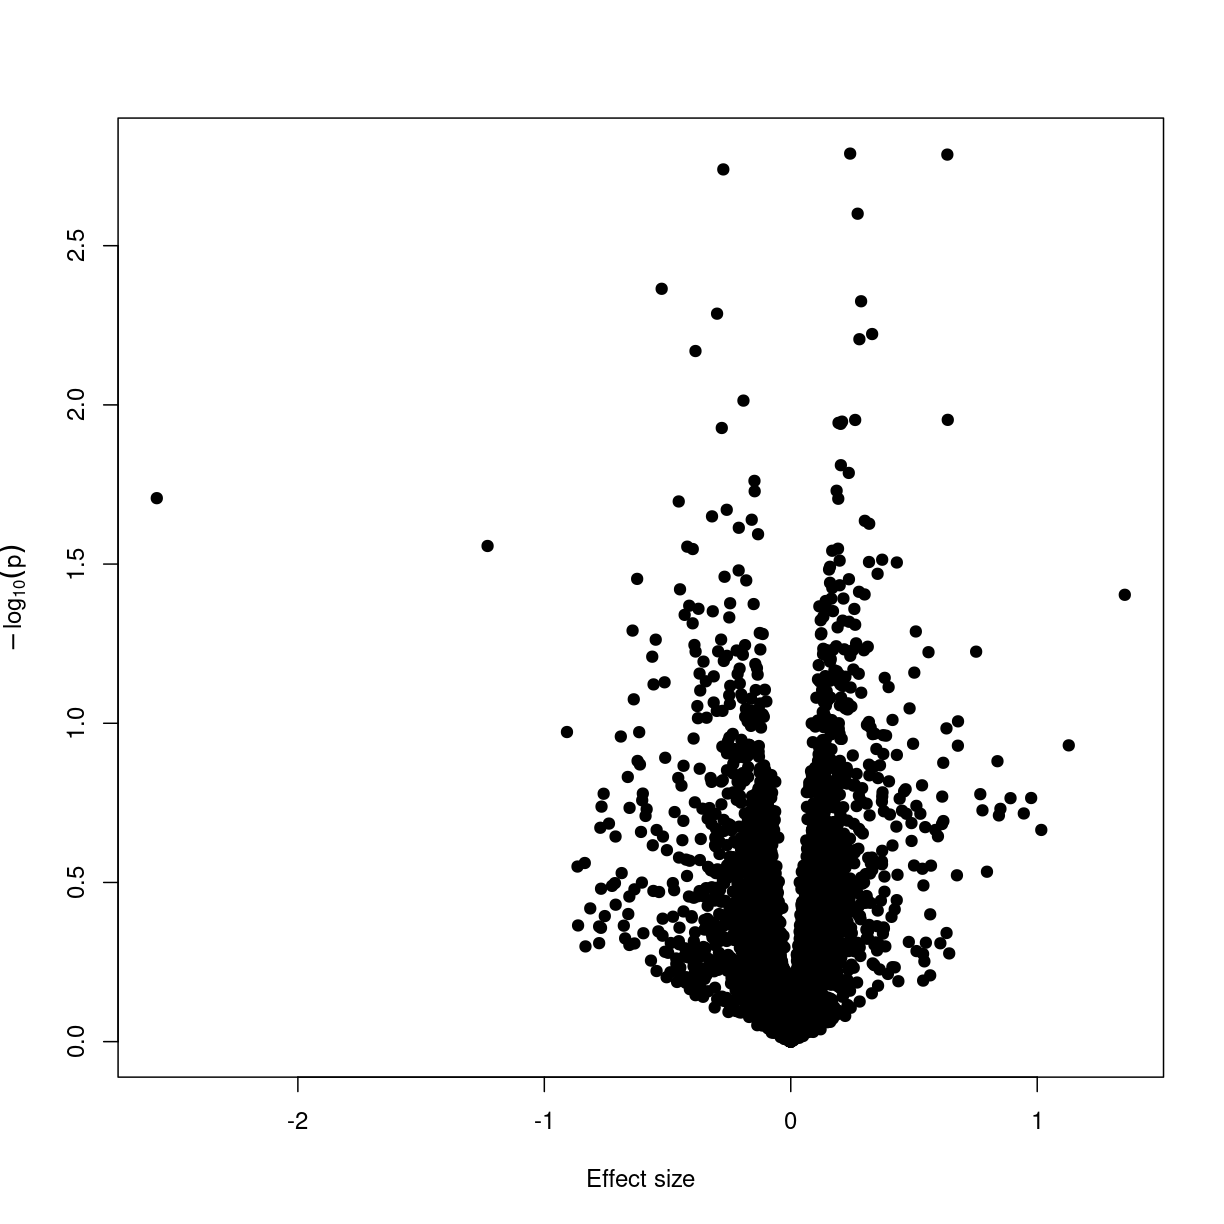
\includegraphics[width=0.5\textwidth]{/home/runner/work/high-dimensional-stats-r/high-dimensional-stats-r/fig/rmd-02-unnamed-chunk-34-1}



\end{frame}

\begin{frame}{A plot of -log10(p) against effect size estimates for a
regression of smoking status against methylation using limma.}
\protect\hypertarget{a-plot-of--log10p-against-effect-size-estimates-for-a-regression-of-smoking-status-against-methylation-using-limma.}{}

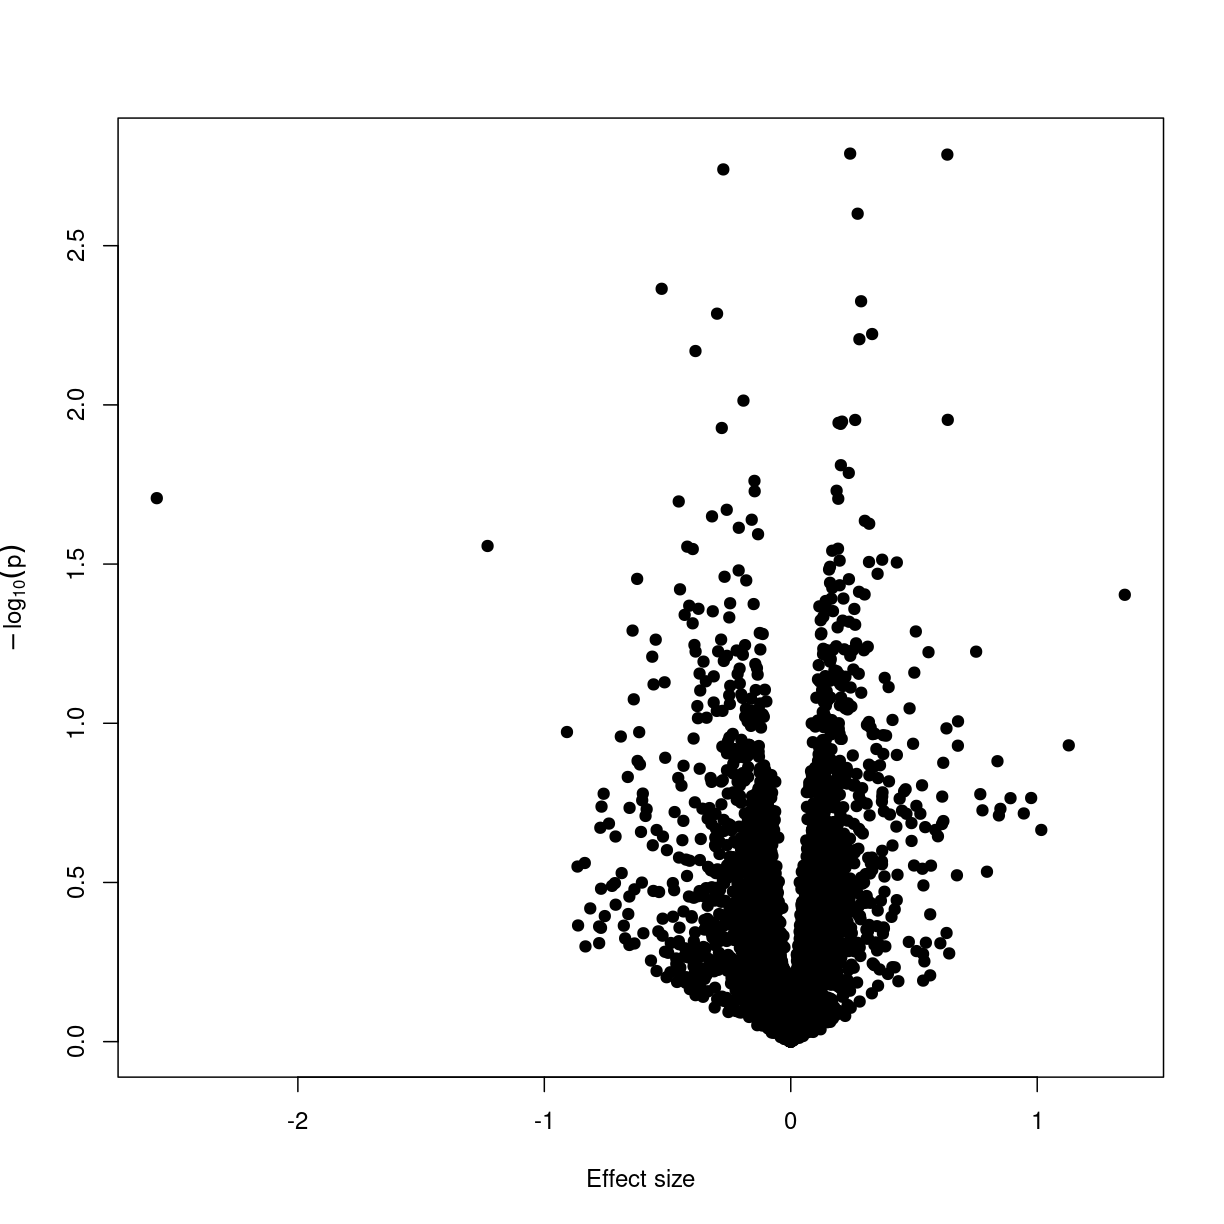
\includegraphics[width=0.5\textwidth]{/home/runner/work/high-dimensional-stats-r/high-dimensional-stats-r/fig/rmd-02-unnamed-chunk-36-1}



\end{frame}

\end{document}
